\documentclass[11pt,a4paper]{article}
\usepackage[T1]{fontenc}
\usepackage{lmodern}
\usepackage{a4wide}
\usepackage[dvips]{graphicx}

\usepackage[
pdfauthor={ ACE Projekt Team },
pdftitle={ Evaluation Algorithms },
pdfcreator={pdftex},
]{hyperref}

\usepackage{sectsty}
\allsectionsfont{\sffamily}

\usepackage{fancyheadings} 
\pagestyle{fancy} 
\lhead{\textsf{\textbf{ACE} \\ \small{a collaborative editor}}}
\chead{}
\rhead{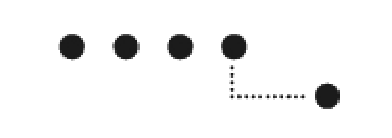
\includegraphics[height=0.875cm,width=3cm]{../../images/logo_BFH.eps}}
\lfoot{}
\cfoot{\textsf{\thepage}}
\rfoot{}
\setlength{\headrulewidth}{0.6pt}
\setlength{\footrulewidth}{0.6pt}
\setlength{\topmargin}{-50pt}
\addtolength{\headheight}{50pt}

\usepackage{colortbl}

\newcommand{\headercol}[2]{\multicolumn{1}{|>{\bfseries\columncolor[gray]{0.82}}p{#1}|}{\textsf{#2}}}
\newcommand{\ace}[0]{\emph{ACE }}



\begin{document}
\setlength{\parindent}{0pt}

\newtheorem{defn}{Definition}

\bibliographystyle{plain}

\begin{titlepage}
\thispagestyle{empty}
  \includegraphics[height=1.5in]{../../images/pix.eps}

  \begin{center}

    {\fontsize{40}{45} \textbf{\textsf{ACE}}} \\
    \textsf{a collaborative editor} \\
        
    \vspace{36pt}
        
    {\huge{\textbf{\textsf{Report Evaluation Network}}}} \\

    \vspace{36pt}

	\textsf{Berne University of Applied Sciences} \\
    \textsf{School of Engineering and Information Technology} \\
    
  \end{center}

  \vfill
  
  \begin{tabular}{ll}
   \hline

   \\

   \multicolumn{1}{>{\bfseries}p{1.5in}}{\textsf{Date:}} &
   \multicolumn{1}{>{}p{4.3in}}{\textsf{14.06.2005}}          \\
   
   \\
   
   \multicolumn{1}{>{\bfseries}p{1.5in}}{\textsf{Version:}}     &   
   \multicolumn{1}{>{}p{4.3in}}{\textsf{0.6}}                 \\

   \\
   
   \multicolumn{1}{>{\bfseries}p{1.5in}}{\textsf{Projectteam:}}                 &
   \multicolumn{1}{>{}p{4.3in}}{\textsf{Mark Bigler (biglm2@hta-bi.bfh.ch)}}  \\
   \multicolumn{1}{>{\bfseries}p{1.5in}}{}                                      &
   \multicolumn{1}{>{}p{4.3in}}{\textsf{Simon R�ss (rasss@hta-bi.bfh.ch)}}    \\
   \multicolumn{1}{>{\bfseries}p{1.5in}}{}                                      &
   \multicolumn{1}{>{}p{4.3in}}{\textsf{Lukas Zbinden (zbinl@hta-bi.bfh.ch)}} \\   
   
   \\
   
   \multicolumn{1}{>{\bfseries}p{1.5in}}{\textsf{Receivers:}}                       &
   \multicolumn{1}{>{}p{4.3in}}{\textsf{Jean-Paul Dubois (doj@hta-bi.bfh.ch)}}       \\
   \multicolumn{1}{>{\bfseries}p{1.5in}}{}                                          &
   \multicolumn{1}{>{}p{4.3in}}{\textsf{Claude Fuhrer (frc@hta-bi.bfh.ch)}}       \\

   \\
   
   \multicolumn{1}{>{\bfseries}p{1.5in}}{\textsf{Location:}}               &   
   \multicolumn{1}{>{}p{4.3in}}{\textsf{Subversion Repository}} \\

   \\  
   
   \hline
  \end{tabular}

\end{titlepage}

\newpage

\tableofcontents
\newpage
\listoftables
\listoffigures
\newpage


\section*{Versionskontrolle}

\begin{table}[!h]
 \begin{tabular}{|l|l|l|l|}
  \hline
  \headercol{0.6in}{Version}         & 
  \headercol{0.8in}{Datum}           &
  \headercol{1.2in}{Verantwortlich}  & 
  \headercol{2.8in}{Bemerkungen}     \\
  \hline
  0.1         & 15.03.2005  & zbinl           &  Erste Version \\
  0.2         & 16.03.2005  & Projektteam     &  �berarbeitung \\
  0.3         & 05.04.2005  & Projektteam     &  �berarbeitung vor Abgabe \\
  \hline
 \end{tabular}
 \caption{Versionskontrolle}
 \label{Versionskontrolle}
\end{table}

\begin{table}[!h]
 \begin{tabular}{|l|l|l|l|l|}
  \hline
  \headercol{0.9in}{}            & 
  \headercol{0.9in}{Stelle}      & 
  \headercol{0.8in}{Datum}       & 
  \headercol{0.6in}{Visum}       & 
  \headercol{2.0in}{Bemerkungen} \\
  \hline
  \textbf{Freigegeben}   & Projektteam &       &       &             \\
  \hline
  \textbf{Genehmigt}     &             &       &       &             \\
  \hline
 \end{tabular}
 \caption{Pr�fung/Genehmigung}
 \label{Pr�fung/Genehmigung}
\end{table}

\newpage


\section{Introduction}
Real-time cooperative editing systems allow multiple users to view and edit the same document at the same time from multiple sites connected by communication networks. Consistency maintenance is one of the most significant challenges in designing and implementing real-time cooperative editing systems. 

\subsection{Preliminaries}
In this section, some basic concepts and terminologies are introduced. Following Lamport\cite{lamport}, we define a causal (partial) ordering relation on operations in terms of their generation and execution sequences as follows.

\begin{defn}
Causal ordering relation $\rightarrow$: \\
Given two operations $O_{a}$ and $O_{b}$ generated at sites $i$ and $j$, then $O_{a}\rightarrow O_{b}$, iff:
\begin{enumerate}
 \item $i=j$ and the generation of $O_{a}$ $j$, then $O_{a}\rightarrow O_{b}$
 \item or $i \neq $j and the execution of $O_{a}$ at site $j$ happened before the 
       genration of $O_{b}$
 \item or there exists an operation $O_{x}$ such that $O_{a}\rightarrow O_{x}$
       and $O_{x}\rightarrow O_{b}$
\end{enumerate}
\end{defn}

\begin{defn}
Dependent and independent operations: \\
Given any two operations $O_{a}$ and $O_{b}$:
\begin{enumerate}
 \item $O_{b}$ is \emph{dependent} on $O_{a}$ iff $O_{a} \rightarrow O_{b}$
 \item $O_{a}$ and $O_{b}$ are \emph{independent} (or \emph{concurrent}), expressed
       as $O_{a} \Arrowvert O_{b}$ iff neither $O_{a}\rightarrow O_{b}$ nor
       $O_{b}\rightarrow O_{a}$
\end{enumerate}
\end{defn}

Intuitively we can say that two operations are dependant if there is a path from the generation of one message to the generation of another message. So for example in figure \ref{fig:example1} operation $O_{1}$ and $O_{3}$ are dependent, that is $O_{1}\rightarrow O_{3}$. Operation $O_{1}$ and $O_{2}$ are \emph{independent}. 


\subsection{Requirements}
The following requirements have been identified for such systems.

\paragraph{Real-time:} The response to local user actions must be quick, ideally as quick as a single-user editor, and the latency for reflecting remote user actions is low (determined by external communication latency only). 

\paragraph{Distributed:} Cooperating users may reside on different machines connected by communication networks with nondeterministic latency.

\paragraph{Unconstrained:} Multiple users are allowed to concurrently and freely edit any part of the document at any time, in order to facilitate free and natural information flow among multiple users.

The requirements for good responsiveness and for supporting unconstrained collaboration have led researchers to adopt a replicated architecture for the storage of shared documents. The shared documents are replicated at the local storage of each participating site. One of the most challenging problem in designing and implementing real-time cooperative editing systems with a replicated architecture is consistency maintenance of replicated documents. 

To illustrate the challenges researchers are facing, consider a scenario in a cooperative editing system with three cooperating sites, as shown in figure \ref{fig:example1}. Suppose that an operation is executed on the local replica of the shared document immediately after its generation, then broadcast to remote sites and executed there in its \emph{original form} upon its arrival.


\subsection{Three inconsistency problems}
Three different inconsistency problems have been identified by {Sun et. al}\cite{sun98a}.

\begin{figure}
 \centering
 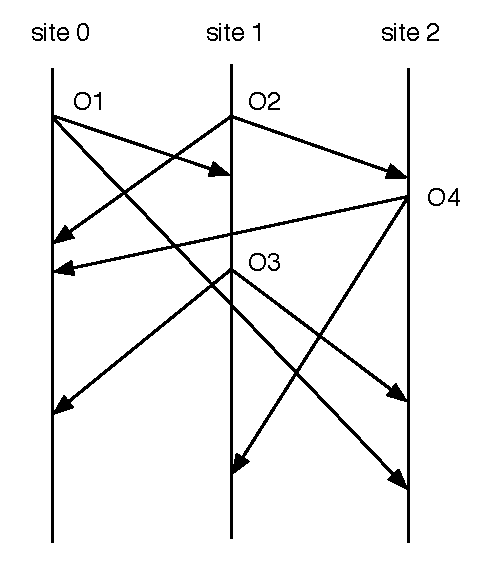
\includegraphics[width=4.68in,height=4.33in]{../../images/example1.eps}
 \caption{A scenarion of a real-time cooperative editing session}
 \label{fig:example1}
\end{figure}

\paragraph{Divergence:}
Operations may arrive and be executed at different sites in different orders, resulting in different final results. As shown in figure \ref{fig:example1}, the four operations in this scenario are execute in the following orders: $O_{1}$, $O_{2}$, $O_{4}$ and $O_{3}$ at site 0; $O_{2}$, $O_{1}$, $O_{3}$ and $O_{4}$ at site 1; and $O_{2}$, $O_{4}$, $O_{3}$ and $O_{1}$ at site 2. Unless operations are commutative, which is generally not the case, final editing results will diverge. The divergence problem can be solved by any serialization protocol, which ensures the final result is the same as if all operations were executed in the same total order at all sites.

\paragraph{Causality violation:}
Due to the nondeterministic communication latency, operations may arrive and be executed out of their natural cause-effect order. As shown in figure \ref{fig:example1}, operation $O_{3}$ is generated after the arrival of $O_{1}$ at site 1, the editing effect of $O_{1}$ on the shared document has been seen by the user 1 at the time $O_{3}$ is generated. Therefore, $O_{3}$ may be \emph{dependent} on $O_{1}$. However, since $O_{3}$ arrives and is executed before $O_{1}$ at site 2, confusion may occure to the system as well as to the user at site 2. For example, if $O_{1}$ is to insert a string into a shared document, and $O_{3}$ is to delete some characters in the string inserted by $O_{1}$, then the execution of $O_{3}$ before $O_{1}$ at site 2 will result in $O_{3}$ referring to a nonexistent context. 

\paragraph{Intention violation:}
Due to concurrent generation of operations, the \emph{actual effect} of an operation at the time of its execution may be different from the \emph{intended effect} of this operation at the time of its generation. As shown in figure \ref{fig:example1}, operation $O_{1}$ is generated at site 0 without any knowledge of $O_{2}$ generated at site 1, so $O_{1}$ is \emph{independent} of $O_{2}$, and vice versa. At site 0, $O_{2}$ is executed on a document state which has been changed by the preceding execution of $O_{1}$. Therefore, the subsequent execution of $O_{2}$ may refer to an incorrect position in the new document state, resulting in an editing effect which is different from the \emph{intention} of $O_{2}$. 

For example, assume the shared document initially contains the following sequence of characters: "'ABCDE"'. Suppose $O_{1}=Insert["'12"',1]$, which intends to insert string "'12"' at position 1, i.e. between "'A"' and "'BCDE"'; and $O_{2}=Delete[2,2]$, which intends to delete the two characters starting from position 2, i.e. "'CD"'. After the execution of these two operations, the \emph{intention-preserved} result (at all sites) should be: "'A12BE"'. However, the actual result at site 0, obtained by executing $O_{1}$ followed by executing $O_{2}$, would be: "'A1CDE"', which apparently violates the intention of $O_{1}$ since the character "'2"', which was intented to be inserted, is missing in the final text, and violates the intention of $O_{2}$ since characters "'CD"', which were intended to be deleted, are still present in the final text.

Even if a serialization-based protocol was used to ensure that all sites execute $O_{1}$ and $O_{2}$ in the same order to get an identical result "'A1CDE"', but this identical result is still inconsistent with the intentions of both $O_{1}$ and $O_{2}$.


\subsection{Operational Transformations}
{Ellis and Gibbs}~\cite{ellis} proposed a new kind of algorithms, called \emph{Operational Transformations} (OT).  These kind of algorithms transform operations, or more specifically their index, to include/exclude other operations.

In general there are two different types of operational transformations, inclusion transformation (IT) and exclusion transformation (ET). All algorithms use inclusion transformation, some use exclusion transformation too.

A transformation function has to be defined for every combination of operations. So for a text editor with the primitive operations insert and delete, there would be a total of four transformations functions for IT and yet another four for ET.

\subsubsection{Definitions}
Conceptually, an operation $O$ is associated with a \emph{context}, denoted as $CT_{O}$, which is the list of operations that need to be executed to bring the document from its initial state to the state on which $O$ is defined. The significance of context is that the effect of an operation can be correctly interpreted only in its own context. 

\begin{defn}
Context equivalent relation $\sqcup$
\end{defn}

Given two operations $O_{1}$ and $O_{2}$, associated with contexts $CT_{O_{1}}$ and $CT_{O_{2}}$ respectively, $O_{1}$ and $O_{2}$ are \emph{context-equivalent} iff $CT_{O_{1}}=CT_{O_{2}}$. Apparently, the context equivalent relation $\sqcup$ is transitive.

\begin{defn}
Context preceding relation $\mapsto$
\end{defn}
Given two operations $O_{1}$ and $O_{2}$ associated with contexts $CT_{O_{1}}$ and $CT_{O_{2}}$ respectively, $O_{1}$ is \emph{context preceding} $O_{2}$ iff $CT_{O_{2}}=CT_{O_{1}} + [O_{1}]$. Note that the contex preceding relation $\mapsto$ is not transitive by definition.

\subsubsection{Inclusion Transformation}
Inclusion Transformation (IT) transforms an operation $O_{1}$ against another operation $O_{2}$ in such a way that the impact of $O_{2}$ is effectively included. 

Most importantly, it was recognized that the correctness of IT relies on the condition that both $O_{1}$ and $O_{2}$ are defined on the same document state so that their parameters are comparable and can be used to derive a proper adjustment to $O_{2}$, i.e. $O_{1} \sqcup O_{2}$.

\subsubsection{Exclusion Transformation}
Exlusion Transformation (ET) transforms an operation $O_{1}$ against another operation $O_{2}$ in such a way that the impact of $O_{2}$ is effectively excluded from $O_{1}$.

Precondition for the exclusion transformation is that $O_{2}$ must contextualy preceed $O_{1}$, i.e. $O_{2} \mapsto O_{1}$.


\subsection{Transformation Properties}
It was shown in \cite{ressel96} that transformation functions must satisfy two conditions, called $TP1$ and $TP2$.

\paragraph{Transformation Property 1:}
The transformation property 1 ensures that the effect of executing $O_{1}$ followed by the transformed request $O_{2}$ is the same as executing request $O_{2}$ followed by the transformed request $O_{1}$. 

\begin{defn}
Transformation Property 1:
$ O_{1} O'_{2} \equiv O_{2} O'_{1} $
\end{defn}

\paragraph{Transformation Property 2:}
Transformation property 1 is a necessary and sufficient condition to ensure that the groupware system with two users is correct. When there are more than two users, the situation is more complex. An operation can be transformed along different, albeit equivalent paths, not necessarily yielding the same result. In the simplest case, an operation can be transformed along the two paths of a simple transformation step. Operation $O_{1}$ may be transformed first with respect to $O_{2}$ and then to $O'_{3}$ yielding $IT(IT(O_{1},O_{2}),O'_{3})$, or it may be transformed first with respect to $O_{3}$ and then to $O'_{2}$ yielding $IT(IT(O_{1},O_{2}),O'_{2})$. Note that different sites might choose different paths for $O_{1}$ to be transformed. So we have to make sure that both paths lead to the same resulting operation:

\begin{defn}
Transformation Property 2: 
$IT(IT(O_{1},O_{2}),O'_{3})$=$IT(IT(O_{1},O_{2}),O'_{2})$
\end{defn}


\section{History}
{Ellis and Gibbs}~\cite{ellis} were the first to propose an \emph{Operational Transformation} algorithm in 1989. The algorithm is called \emph{dOPT} and is implemented in the \emph{Grove} system. Soon however a flaw was discovered in the original \emph{dOPT} algorithm (by Cormack\cite{cormack95a}). The scenario where \emph{dOPT} failed is called the \emph{dOPT} puzzle. Ressel\cite{ressel96} proposed a new algorithm \emph{adOPTed} in 1996 that solved the original \emph{dOPT} puzzle. {Sun et. al}\cite{sun98a} proposed another algorithm called \emph{GOT} that similarly to \emph{adOPTed} solved the \emph{dOPT} puzzle. {Sun et. al}\cite{sun98b} developed some transformation functions for string-wise operations.

Later research groups\cite{imine03}\cite{imine04} proved the transformation functions of both Ressel\cite{ressel96} and Sun\cite{sun98a} to fail to hold TP2 in certain situations. They proposed new transformation functions they developed using a theorem prover. 

Proving the transformation property 1 (TP1) seems to be rather straightforward. However, proving that a given transformation function holds TP2 appears to be difficult. There are over 100 cases that have to be analyzed (according to {Imine et. al}\cite{imine04}). Imine et. al shows that many proposed transformation functions do not hold TP2. 

Recently, two different ways have been taken to deal with the TP2 problem. One kind of algorithms try to avoid the need to comply with TP2 altogether (SOCT2~\cite{suleiman97}, GOT~\cite{sun98a}, SOCT3/4~\cite{suleiman00}, TIBOT\cite{tibot} and NICE~\cite{sun02}). Other research groups try to correct the problems in the original transformation functions of GOTO\cite{sun98b} and adOPTed\cite{ressel96}. 


\section{Algorithms}
In this section we give an overview of all the \emph{Operational Transformation} algorithms we have found so far.

\subsection{Introduction}
It is important to note, that a complete functioning OT algorithm usually consists of two parts. One part, the control algorithm, is application independent. The other part is the set of transformation functions (IT and maybe ET), which is application dependent. As noted earlier, for every pair of operations there must be one (when the algorithm uses ET two) transformation function. For two operations (e.g. insert and delete) this results in four transformation functions. Operations are highly application dependent. A text editor has different operations than a whiteboard application.

\subsection{dOPT}
\label{algo:dopt}

\emph{dOPT} (Distributed Operational Transformation) is the first operational transformation algorithm developed by {Ellis and Gibbs}\cite{ellis} in 1989. It was soon discovered that in some situations the document replicas did not converge. This situation is known as the \emph{dOPT} puzzle.

The algorithm fails in cases where there is more than one concurrent operation from a user. Gormack\cite{cormack95a} detected this case and proposed a new algorithm (see \ref{algo:ccu}) that is only suitable for two sites connected by a point-to-point communication channel. He stated that there does not appear to be a simple and efficient correction to \emph{dOPT} that maintains its suitability for broad-cast operations.

However Gormack showed in \cite{cormack95b} that using several point-to-point communication channels forming a tree it is possible to derive a consistent solution for an arbitrary number of sites.

\subsubsection{Properties}
\begin{itemize}
 \item algorithm is incorrect
 \item uses state vectors to maintain causal ordering
 \item uses linear history buffer (called request log)
 \item architecture: fully replicated
\end{itemize}

\subsection{CCU}
\label{algo:ccu}

CCU (a Calculus for Concurrent Update) derives from the \emph{dOPT} (see \ref{algo:dopt}) algorithm. It was developped by Gordon V.Cormack in 1995 that discovered earlier \cite{cormack95a} that \emph{dOPT} is incorrect. 

The algorithm specifies a concurrent model based on a sequential model augmented with definitions of all possible pairs of elementary operations (updates). The concurrent model is implemented by a set of objects: one for each source of events.

Although there is a description of the algorithm in \cite{cormack95b}, many implementation details are left out. The only information is given is that the simplest n-site algorithm is a star built from multiple versions of the 2-site implementation.

Interestingly no references to this algorithm are found in the research material from other researchers. 

\subsubsection{Properties}
\begin{itemize}
 \item correctness never confirmed by other reaserchers
 \item uses state vectors to maintain causal ordering
 \item architecture: semi-replicated (central server)
\end{itemize}

\subsection{Jupiter}
\label{algo:jupiter}

\emph{Jupiter} is a multi-user, multimedia virtual world intended to support long-term remote collaboration. In particular, it supports shared documents, shared tools, and, optionally, live audio/video communication. The low-level communication facilities are described in \cite{jupiter95}.

The state of the \emph{Jupiter}, including application code written by users, is stored and (for code) executed in a central server shared by all users. This architecture was chosen to support multiple client platforms and high-latency networks. Clients and servers communicate in terms of high-level widgets and user events.

\emph{Jupiter}'s algorithm is derived from \emph{dOPT}. The centralized architecture and thus the reduction of point-to-point connections allows them to simplify the \emph{dOPT} algorithm. Several point-to-point connections are used to build a tree-structured $n$-site algorithm.

\emph{Jupiter} solves the \emph{dOPT} puzzle. It uses a two dimensional state space instead of a linear history buffer (request log) to save operations. It transforms saved messages when there are incoming messages. Unfortunately, simply transforming saved messages does not work for the $n$-way case, since the next message can come from a third site that is in an inconvenient message state.

The algorithm labels each message with the state the sender was in just before the message was generated. The recipient uses these labels to detect conflicts. Two concurrent messages have to be transformed, but they can only be transformed  when they were generated from the same state of the document. Otherwise, special handling is required.


\subsubsection{Properties}
\begin{itemize}
 \item seems to be correct
 \item uses state vectors to decide causality relations
 \item architecture: semi-replicated (central server)
 \item uses multiple 2-way synchronization protocols to create a n-way protocol
\end{itemize}

\subsection{NetEdit Consistency Algorithm}
\label{algo:netedit}

\emph{NetEdit} is a collaborative text editor (\cite{netedit}) that uses a replicated architecture with processing and data distributed across all clients. It uses an $n$-way synchronization protocol derived from the algorithm of the \emph{Jupiter} (see \ref{algo:jupiter}) collaboration system. The algorithm is called \emph{NetEdit Consistency Algorithm}.

The 2-way synchronization protocol developed for \emph{Jupiter} was the starting point. That algorithm was extended to a multi-way protocol using multiple 2-way connections. All the clients maintain a state-space graph. This state-space is used to maintain information where the other is in the editing process. Both client and server pass through this state space as they process messages.

The algorithm labels each message with the state the sender was in just before the message was generated. The recipient uses these labels to detect conflict. Two concurrent messages have to be transformed, but they can only be transformed  when they were generated from the same state of the document. Otherwise, special handling is required.

It is not clear how this algorithm differs from \emph{Jupiter} as \emph{Jupiter} was obviously extended to an n-way synchronization protocol using a similar (the same?) approach.


\subsubsection{Properties}
\begin{itemize}
 \item seems to be correct
 \item uses state vectors to decide if operations are concurrent
 \item architecture: semi-replicated (central server)
 \item uses multiple 2-way synchronization protocols to create a n-way protocol
\end{itemize}


\subsection{adOPTed}
\label{algo:adopted}

\subsection{GOT}
\label{algo:got}

\subsection{GOTO}
\label{algo:goto}

\subsection{SOCT2}
\label{algo:soct2}

\subsection{SOCT3}
\label{algo:soct3}

Verifying that a given set of transformation functions satiesfies transformation property 2 (TP2) is not trivial. There are over a hundred cases to be checked depending on the various parameters. So the inventors of \emph{SOCT3} and \emph{SOCT4} (see \ref{algo:soct4}) decided to go a different way in order that  TP2 must not hold (\cite{suleiman00}).

They propose the implementation of a global serialization order such that the operations can be delivered in this order. The global serialization order is achieved by the use of a sequencer (see \ref{sequencer}). A sequencer is an object which delivers continously growing positive integer values, called timestamps. A timestamp is obtained through a call to a function \emph{Ticket}.

A local operation $O$ is executed immediately to respect the real-time constraint. Next, the call to the function \emph{Ticket} returns a timestamp $N_{O}$ which is assigned to the operation. The quadruplet $<O,S_{O},V_{O},N_{O}>$ is then broadcast where $V_{O}$ is the state vector associated with $O$ and $N_{O}$.

The reception procedure ensures a sequential delivery of all operations with respect to the ascending order of the timestamps. Upon receiving an operation it delays its delivery until all operations with lower timestamps have been received and delivered. The state vector is of no use for the reception procedure, but it enables to determine which operations are concurrent to $O$ during the integration step.

\emph{SOCT3} uses both inclusion transformation IT (called forward transposition) and exclusion transformation ET (called backward transposition) in the integration step. For details, see \cite{suleiman00}.


\subsubsection{Properties}
\begin{itemize}
 \item uses state vectors to determine causal relations
 \item uses linear history buffer (called history)
 \item architecture: fully replicated
 \item uses a unique global ordering to abandon TP2 (by using a sequencer)
 \item no known user undo algorithm
\end{itemize}

\subsection{SOCT4}
\label{algo:soct4}

In \emph{SOCT4} (\cite{suleiman00}) as in \emph{SOCT3}, the operations are ordered globally using a timestamp given by a sequencer. They are then delivered on each site in this order thanks to the sequential reception. The originality of \emph{SOCT4} comes from the fact that inclusion transformation (called forward transposition) that takes into account concurrent operations are now made by the generator sites of the operations. According to \cite{suleiman00} this results in three major advantages:

\begin{enumerate}
 \item the receiver site does not have to separate history anymore; 
       thus backward transposition becomes unecessary
 \item the received operation can be stored as it is in the history
       without further transformation
 \item state vectors are no longer needed
\end{enumerate}

To achieve this, the broadcast of an operation must be deferred until it has been assigned a timestamp and all the operations which precede it according to the timestamp order have been received and executed. As usual, local operations are executed immediately without delay.


\subsubsection{Properties}
\begin{itemize}
 \item does not need any state vectors
 \item architecture: fully replicated
 \item uses a unique global ordering to abandon TP2 (by using a sequencer)
 \item no exclusion transformation needed
 \item no known user undo algorithm
\end{itemize}


\subsubsection{Sequencer}
\label{sequencer}
As noted before, both \emph{SOCT3} and \emph{SOCT4} use sequencer to globally serialize operations. In \emph{SOCT4} operations are broadcast sequentially. This makes collaboration difficult when the propagation delay of an operation on the network is high. This characteristic makes \emph{SOCT4} particularly adapted to fast networks.

More information about sequencers can be found in \cite{reed79}. Various methods for implementing sequencers are described in \cite{lelann78} (circulating sequencers) and \cite{banino79} (replicated sequencers).

\subsection{SDT}
\label{algo:sdt}

The algorithm \emph{SDT} was presented in 2004 by Du Li and Rui Li \cite{sdt}. They detected defects in existing inclusion transformation and exclusion transformation functions. The proposed solution (\emph{SDT}) tries to fix these.

\subsubsection{Defects of traditional transformation functions}
The problem is related to inclusion transformation between two insert operations and one delete operation with close position parameters. In some of these cases, the result of inclusion transformation is not deterministic. 

\paragraph{Example: } Given the initial document state ''abc''. The three editing sites 1, 2 and 3 generate $O_{1} = insert(''1'',2)$, $O_{2} = insert(''2'',1)$ and $O_{3} = delete(''b'',1)$ respectively. The three operations are independent. Now consider what happens at site 3. After the deletion of character ''b'' at position 1 the document state becomes ''ac''. The next message arriving is then $O_{2}$ which inserts ''2'' at position 1. The resulting document state is ''a2c''. The next operation $O_{1}$ arrives at site 3 and is transformed against $O_{3}$ and then $O_{2}$. The result of the second transformation is non-deterministic. It could be $insert(''1'',1)$ or $insert(''1'',2)$. However, the original intention of $O_{1}$ is to insert ''1'' after ''b'' and the intention of $O_{2}$ is to insert ''2'' before ''b''. Then ''1'' should appear after ''2'' in the resulting document state (''a21c''). So depending on the chosen priority scheme, the result could be violating the intention of the original operations. Another even more severe problem results from the fact, that the document state of site 3 could diverge from site 1 and 2. A similar problem arises with traditional exclusion transformation functions.

The conventional transformation functions use the site id as priority scheme if two inserts happen at the same position. This was identified as the source of the problems as described above by Du Li and Rui Li. This new algorithm tries to delay the use of site ids.


\subsubsection{Proposed Solution}
The algorithm works conceptually as follows. For each operation the original intention is recovered by computing its $\beta$ value against a well-known document state (the latest synchronization point). Then in performing inclusion transformation, the $\beta$ values are compared. An algorithm to compute $\beta$ is given in the paper. The approach is based on a new concept called state difference, hence the name \emph{SDT} (state difference transformation).

The user intention is always achieved through performing operations that generate certain effects on a given document state. The effect of an operation $O$ on its definition context is trivially itself, either to insert or delete a character. However, the effect of operation $O$ on $S_{i}$ is not as obvious if $S_{i}$ precedes the definition context. To characterize the effect of an operation on a prior document state more accurately, two notations $\beta$ and $\delta$ are introduced.

Read \cite{sdt} for a general overview and \cite{li03} for the implementation details. The former document does not specify important implementation details (e.g. it is not explained how to obtain the \emph{latest synchronization point}). We did not read \cite{li03} because \emph{SDT} was proved incorrect \cite{imine04} and we did not find the document on the Internet.

\subsubsection{Properties}
\begin{itemize}
 \item transformation functions must hold TP2
 \item no undo mechanism
 \item proposed IT/ET functions proved wrong by Imine et. al \cite{imine04}, 
       i.e. they do not hold TP2 in all cases
 \item architecture: replicated, multicast
\end{itemize}




\subsection{TIBOT}
\label{algo:tibot}


\subsection{NICE}
\label{algo:nice}

Haifeng Shen and Chengzhen Sun devised a new operational transformation control algorithm in combination with a notification component in 2002 \cite{sun02}. In this paper they describe a flexible notification framework that can be used to implement a wide range of notification strategies used in collaborative systems.

In the proposed framework, the notification policy that determines when and what to notify is separated from the notification mechanism that determines how to notify. The parameters \emph{frequency} and \emph{granularity} are provided to define various notification policies. 

The frequency parameter determines the \emph{when} aspect of notification, that is, when a notification is propagated/accepted. The granularity parameter determines the \emph{what} aspect of notification, that is, which updates are going to be propagated/accepted. Further there can be a separate policy for input and output direction.

The notification mechanism determines the \emph{how} aspect. Both outgoing and incoming messages are put in distinct buffers (input buffer IB and output buffer OB). An outgoing notification executor (ONE) and an incoming notification executor (INE) are needed to carry out various outgoing and incoming notification policies respectively.

A very important component in the notification mechanism is the notification propagation protocol (NPP), which is needed for propagating updates from the OB at the notifying site to the IB at the notified site.

The notifications are contextually serialized. This is achieved by use of a central notification server, which acts as a centralized serialization point and message relaying agent (all messages pass through this central server). 


\subsubsection{Notification Propagation Protocol}
Before propagating a notification, the notifying site sends a \emph{Token-Request} message to the \emph{Notifier}, waiting for the \emph{Token-Grant} message from the \emph{Notifier}. After being granted the token, the site propagates the notification piggybacked with the \emph{Token-Release} message to the \emph{Notifier}. When the \emph{Notifier} receives the notification and the \emph{Token-Release} message, it forwards the notification to all interested sites. By using the notifier as a message relaying agent, causal relationships among notifications are automatically guaranteed.

This sequential propagation simplifies concurrency control. However it is also inefficient for supporting notification policies for meeting real-time collaboration needs. For propagating one notification that may contain only one operation, three extra messages have to be sent.


\subsubsection{Concurrent Propagation}
So the proposed solution consists of a protocol that allows a site to propagate its notification without first requesting a token, thus effectively eliminating the \emph{Token-Request} message. This operation propagation protocol is called \emph{SCOP} (symmetric contextually-serialized operation propagation). 


\subsubsection{Properties}
The transformation control algorithm is called \emph{SLOT} (symmetric linear operation transformation). Together with the \emph{SCOP} protocol it has the following properties.

\begin{itemize}
 \item architecture: semi-replicated (uses central notification server)
 \item no state vectors needed
 \item no exclusion transformation (ET)
 \item free of transformation property 2 (TP2)
\end{itemize}

The reason why \emph{SLOT} is free of TP2 is that under no circumstance an operation could be transformed against the same pair of operations in different orders. The operation are always ordered uniquely.




\newpage

\appendix
\section{ Appendix }
code fragments

\newpage
\bibliography{ace}

\end{document}



























